\section{Secuencias}\label{sec:uc0}


\subsection{Administrador}\label{sec:uc0}
\subsubsection{Borrar partida de un usuario}
\begin{center}
	  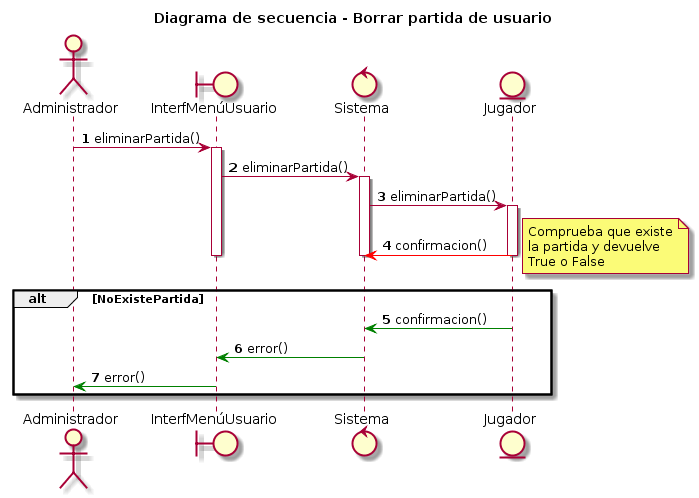
\includegraphics[width=0.9\textwidth]{./imatges/administrador/Borrar_partida_de_usuario.png}
\end{center}
Para borrar una partida, desde el administrador se llama a la función eliminarPartida hasta Jugador, donde se verificará si existe la partida o no, en el caso que exista la partida, la función devuelve al sistema True y en caso contrario False. \\
	Una vez el sistema ha recibido la confirmación, envía un error hasta el administrador.

\subsubsection{Crear una cuenta}
\begin{center}
  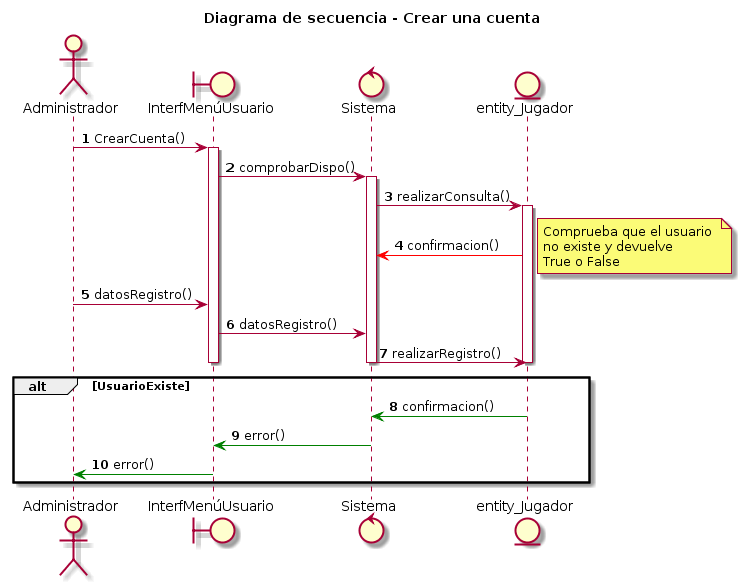
\includegraphics[width=1\textwidth]{./imatges/administrador/Crear_una_cuenta.png}
  \end{center}
  Para crear una cuenta, el administrador llama a la función CrearCuenta() a la Interfície del Menú del Usuario, el cual comprobará la disponibilidad, y el Sistema realiza una Consulta a la Entidad del Jugador para comprobar si el usuario ya existe o no. \\
  La confirmación que se envia al Sistema será True en el caso que se pueda crear la cuenta (el usuario no exista previamente) y False en el caso en el que el usuario ya esté registrado.
  \\Si el usuario puede crearse la cuenta, el administrador llama a la función datosRegistro() a la Interfície del Menú del Usuario, y este al Sistema. El Sistema realizará el Registro hasta la Entidad el Jugador.
  \\En el caso contrario (el administrador no puede crear la cuenta), una vez se realiza la confirmación hasta el Sistema, este envía un error hasta el Administrador, pasado por la ïnterfície del Menú del Usuario.
  
\subsubsection{Crear mapa}
\begin{center}
  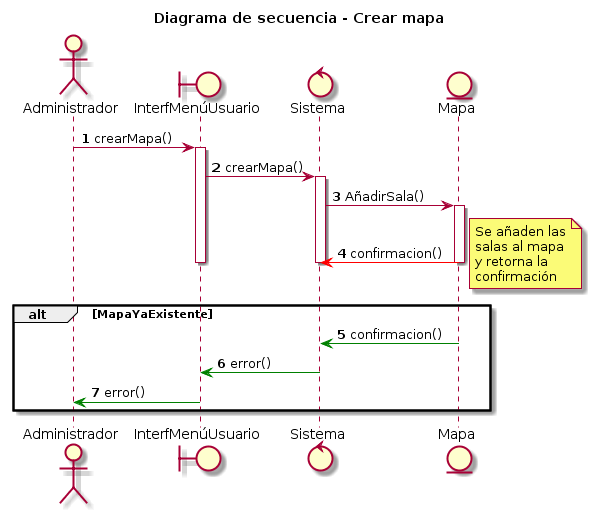
\includegraphics[width=1\textwidth]{./imatges/administrador/Crear_mapa.png}
  \end{center}
  En el caso de querer crear una cuenta, el Administrador llama a la función crearMapa hasta la Interfície del Menú del Usuario y este hasta el Sistema. Del sistema llegamos al Mapa mediante la función AñadirSala() donde de añadirán la salas al mapa y retorna la confirmación hacia el Sistema. Si el mapa ya existe, des de Sistema se envía un error hacia la Interfície del Menú del Usuario, y de este al Administrador.
  
\subsubsection{Eliminar cuanta de usuario}
\begin{center}
  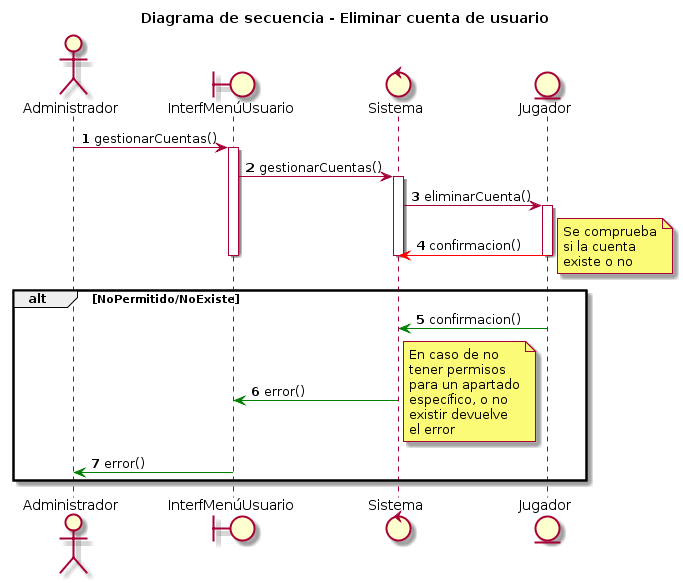
\includegraphics[width=0.9\textwidth]{./imatges/administrador/Eliminar_cuenta_de_usuario.png}
  \end{center}
  Para eliminar una cuenta de usuario, del Administrador llegamos al Sistema, mediante la función gestionarCuentas a través de la Interfície del Menú del Usuario. El sistema llama a la función eliminarCuenta llegando al Jugador, donde de comprueba si la cuenta existe o no.
  \\A continuación se retorna la confirmación hasta el Sistema. Si la cuenta no existe o no se tienen los permisos, se devuelve un error hacia el Administrador a través de la Interfície del Menú del Usuario.
  
\subsubsection{Modificar datos de la cuenta}
\begin{center}
  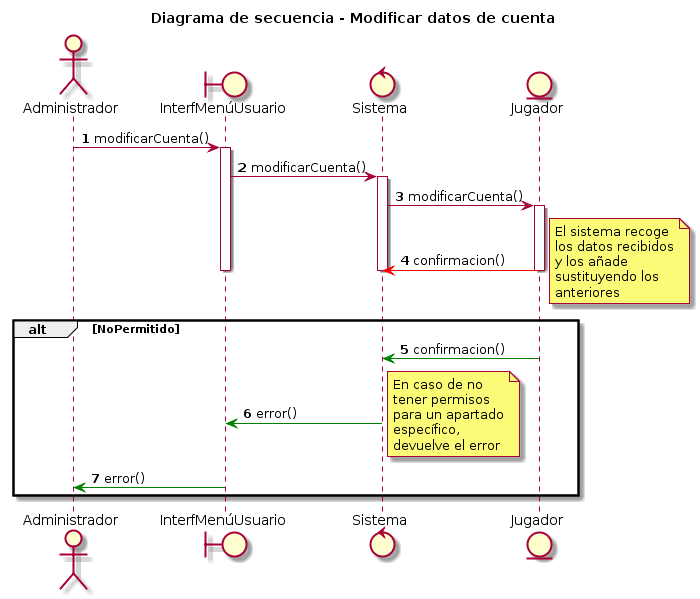
\includegraphics[width=0.9\textwidth]{./imatges/administrador/Modificar_datos_de_cuenta.png}
  \end{center}
  Como vemos en el siguiente diagrama de Secuencia para modificar los datos de una cuenta, el Administrador a partir de la función modificarCuenta() llega al Jugador pasando por la Interfície del Menú del Usuario y el Sistema
  \\A continuación el Sistema recoge los datos recibidor para añadirlos o sustituirlos. Posteriormente, se envía la confirmación al Sistema. En el caso que no se tenga permisos para un apartado específico el Administrador recibirá un error enviado por el Sistema pasando por la Interfície del Menú del Usuario.
  
\subsubsection{Modificar mapa}
\begin{center}
  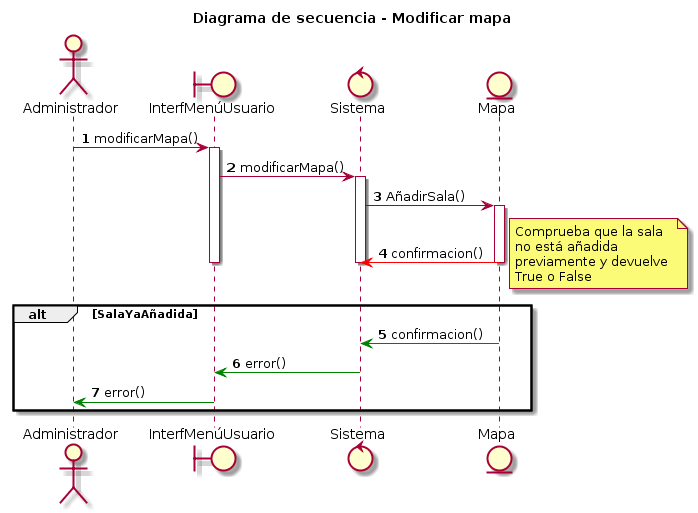
\includegraphics[width=0.9\textwidth]{./imatges/administrador/Modificar_mapa.png}
  \end{center}
  Para modificar un mapa, el Administrador llama a la función modificarMapa() pasando per la Interfície del Menú del Usuario hasta llegar al Sistema. Este llegará hasta Mapa a través de AñadirSala().
  \\Posteriormente, se comprueba si la sala ya estaba añadida previamente, y devuelve True o False mediante la confirmación hasta el Sistema. Si la sala no estaba añadida, el Sistema envía un error al Administrador pasando por la Interfície del Menú del Usuario.
  
\subsubsection{Modificar ranking}
\begin{center}
  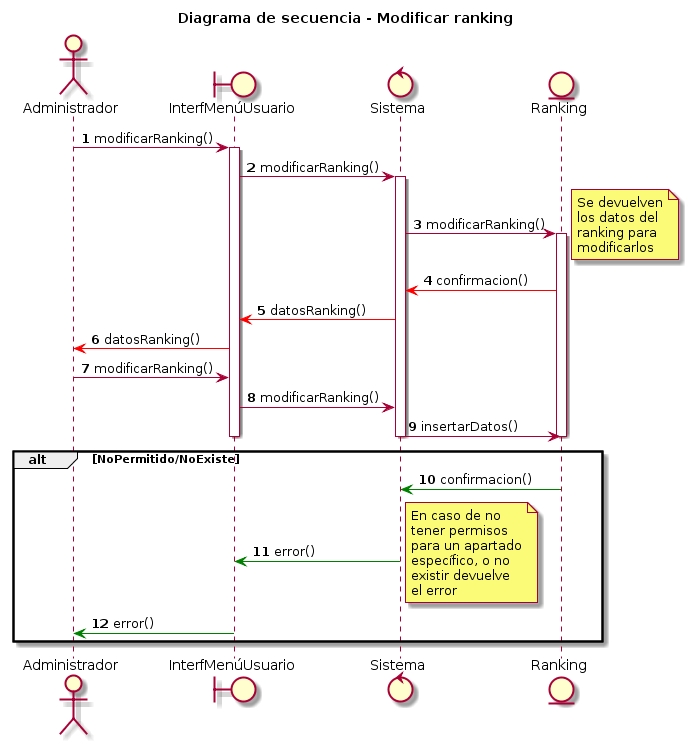
\includegraphics[width=0.8\textwidth]{./imatges/administrador/Modificar_ranking.png}
  \end{center}
  Para modificar un ranking, el Administrador llega al Ranking mediante la función modificarRanking() pasando por la Interfície del Menú del Usuario y el Sistema.
  \\A continuación se devuelve la confirmación hasta el Sistema. En el caso que sea posible la modificación, el Sistema enviará al Administrador los datos del Ranking, pasando por la Interfície del Menú del Usuario. Seguidamente, el Administrador llama modificarRanking() hacia la Interfície del Menú del Usuario y de esta hacia el Sistema. El Sistema insertará los Datos al Ranking.
  \\Si la confirmación es negativa (no se tienen los permisos necesarios o no existe el ranking), el Sistema envía un error hacia el Administrador pasando por la Interfície del Menú del Usuario.
  
\subsubsection{Ver usuarios en línea}
\begin{center}
  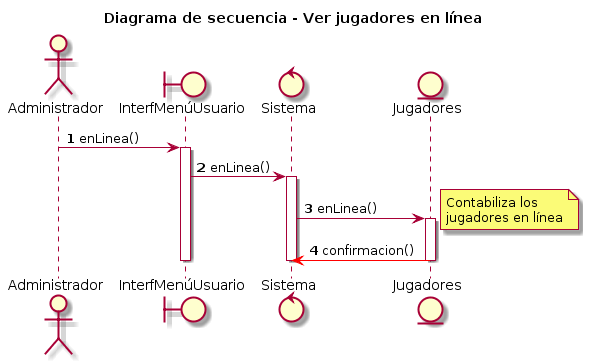
\includegraphics[width=0.9\textwidth]{./imatges/administrador/Ver_usuarios_en_linea.png}
  \end{center}
	En el caso de querer ver los usuarios en línea el Administrador llega hasta los Jugadores mediante la función enLinea() pasando por la Interfície del Menú del Usuario y el Sistema. A continuación se cuentan todos los jugadores en línea, y posteriormente, se envía la confirmación al Sistema.


\subsection{Jugador}\label{sec:uc0}
\subsubsection{Consultar ranking}
\begin{center}
  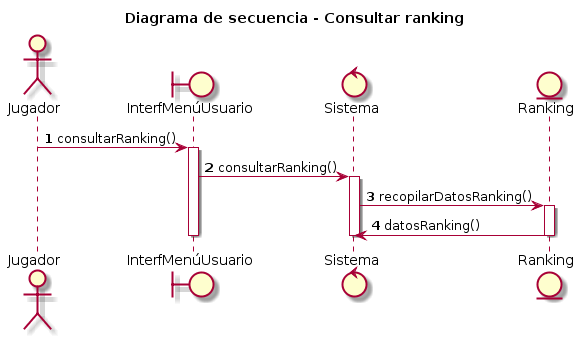
\includegraphics[width=0.9\textwidth]{./imatges/jugador/Consultar_ranking.png}
  \end{center}
  Si se quiere consultar el ranking el Jugador llama a consultarRanking() hasta la Interfície del Menú del Usuario y de esta al Sistema. El sistema recopilar todos los datos del Ranking. El ranking, le devuelve todos los datos al sistema.

\subsubsection{Continuar partida}
\begin{center}
  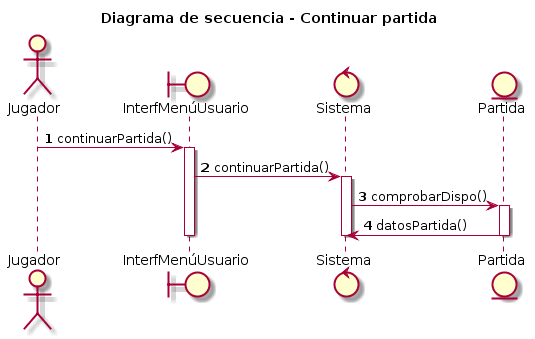
\includegraphics[width=0.9\textwidth]{./imatges/jugador/Continuar_partida.png}
  \end{center}
  El diagrama de secuencia que vemos es necesario para continuar una partida. El Jugador llama a la función continuarPartida() hasta el Sistema pasando por la Interfície del Menú del Usuario. A continuación se comprueba la disponibilidad. Para finalizar, la Partida le envia los datos de la Partida al Sistema.
  
\subsubsection{Crear una cuenta}
\begin{center}
  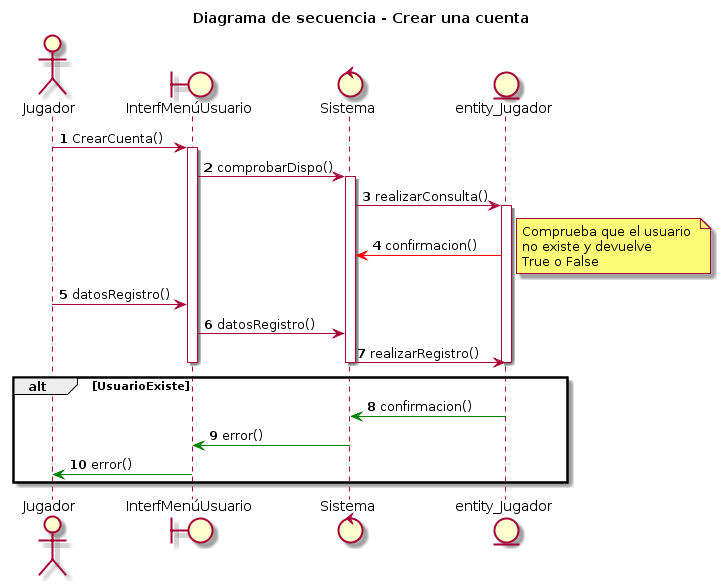
\includegraphics[width=0.9\textwidth]{./imatges/jugador/Crear_una_cuenta.png}
  \end{center}
  Para crear una cuenta el Jugador accede a la Interfície del Menú del Usuario a partir de la función CrearCuenta(), esta comprueba la disponibilidad al Sistema y se realiza la consulta a la Entidad del Jugador, donde se verifica si la cuenta ya existe o no y retorna True o False al Sistema a través de la confirmación.
  \\Si la cuenta no existe, el Jugador envía los datos del Registro hacia el Sistema a través de la Interfície del Menú del Usuario. Finalmente, el Sistema realiza el Registro.
  \\Si la cuenta ya existía previamente, el Sistema envía un error al Jugador pasando por la Interfície del Menú del Usuario.
  
\subsubsection{Eliminar partida}
\begin{center}
  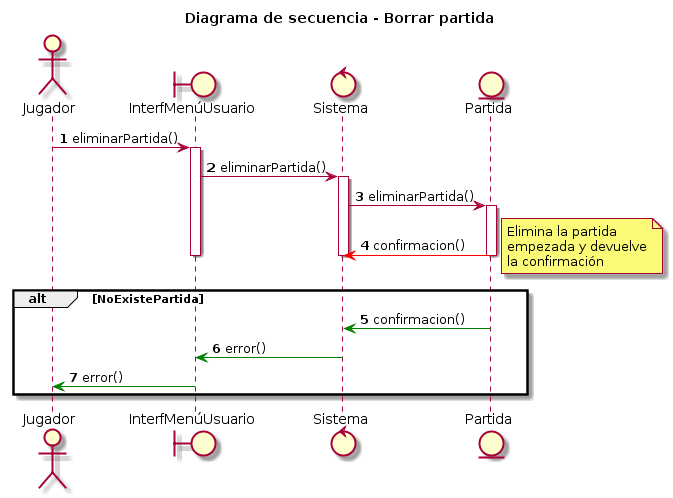
\includegraphics[width=0.9\textwidth]{./imatges/jugador/Eliminar_partida.png}
  \end{center}
  Cuando queremos eliminar una cuenta, el Jugador llama a la función eliminarPartida() hasta Partida, pasando por la Interfície del Menú del Usuario y el Sistema. A continuación se elimina y se envía una confirmación al Sistema.
  \\Si la partida no existía, posteriormente de la confirmación, se envía un error hasta el Jugador a través de la Interfície del Menú del Usuario.
 
\subsubsection{Empezar partida}
\begin{center}
  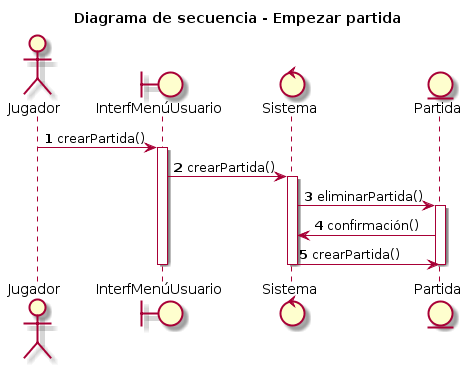
\includegraphics[width=0.9\textwidth]{./imatges/jugador/Empezar_partida.png}
  \end{center}
  A continuación se muestra el diagrama de secuencia para empezar una partida, en este caso, el Jugador accede a la función crearPartida() hasta llegar a Partida, pasando por la Interfície del Menú del Usuario y el Sistema.
  
\subsubsection{Guardar partida}
\begin{center}
  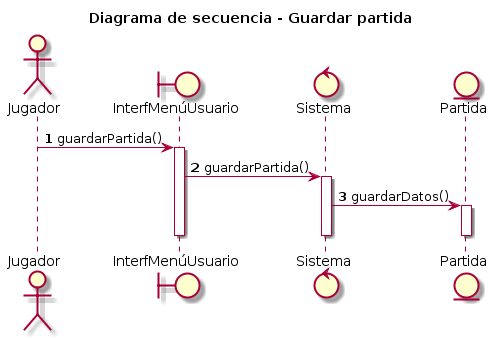
\includegraphics[width=0.9\textwidth]{./imatges/jugador/Guardar_partida.png}
  \end{center}
  Para guardar una partida, el Jugador llama a la función guardarPartida() hasta el Sistema mediante la Interfície del Menú del Usuario, el Sistema guarda los datos a la Entidad Partida.

\subsubsection{Hacer login}
\begin{center}
  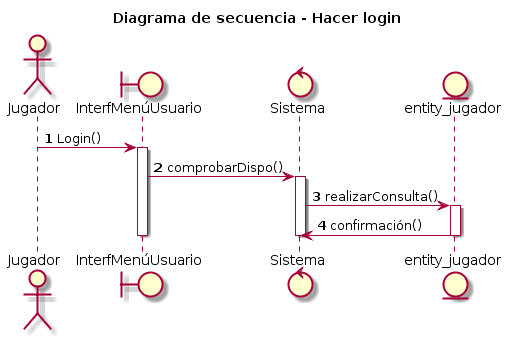
\includegraphics[width=0.9\textwidth]{./imatges/jugador/Hacer_login.png}
  \end{center}
  Para hacer el login, el Jugador accede a la Interfície del Menú del Usuario a través de Login(), la Interfície del Menú del Usuario comprueba la disponibilidad. A continuación el Sistema realiza la consulta a la entidad del Jugador. Para finalizar el login, se le envía la confirmación al Sistema.

\subsubsection{Menú de movimientos}
\begin{center}
  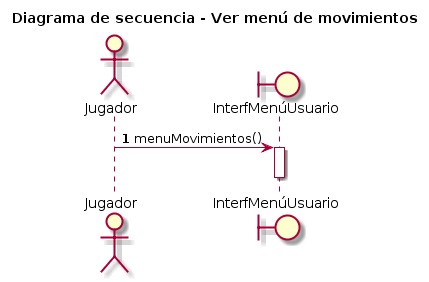
\includegraphics[width=0.9\textwidth]{./imatges/jugador/Menu_de_movimientos.png}
  \end{center}
  El diagrama de secuencia para ver el menú de movimientos como vemos es muy sencillo, simplemente el Jugador accede a la Interfície del Menú del Usuario mediante menuMovimientos().

\subsubsection{Modificar datos de la cuenta}
\begin{center}
  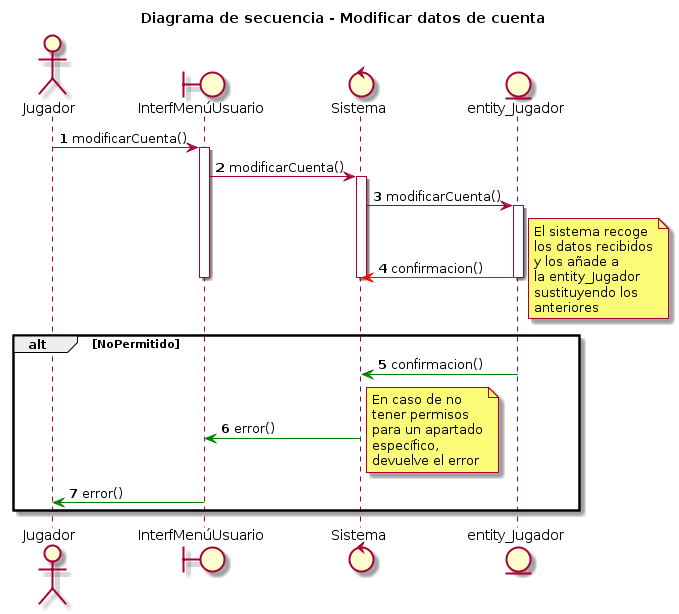
\includegraphics[width=0.9\textwidth]{./imatges/jugador/Modificar_datos_de_cuenta.png}
  \end{center}
  Para modificar datos de la cuenta, el Jugador llama a la función modificarCuenta() hasta la entidad Jugador, pasando por la Interfície del Menú del Usuario y el sistema. El sistema reúne todos los datos recibidos y los añade o los sustituye. Posteriormente envía la confirmación al sistema. Si no se tienen los permisos requeridos, el sistema devuelve un error hasta el Jugador.

\subsubsection{Salir del juego}
\begin{center}
  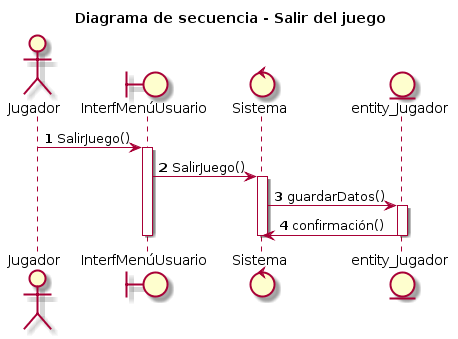
\includegraphics[width=0.9\textwidth]{./imatges/jugador/Salir_del_juego.png}
  \end{center}
  Por último, para salir del juego, el Jugador accede al Sistema mediante la función SalirJuego() pasando por la Interfície del Menú del Usuario. El Sistema guarda los datos en la entidad del Jugador. Finalmente, se se envía la confirmación al Sistema.

